\begin{frame}{Mais à l'école?}
  \begin{columns}
    \column{0.4\textwidth}
      \begin{center}
        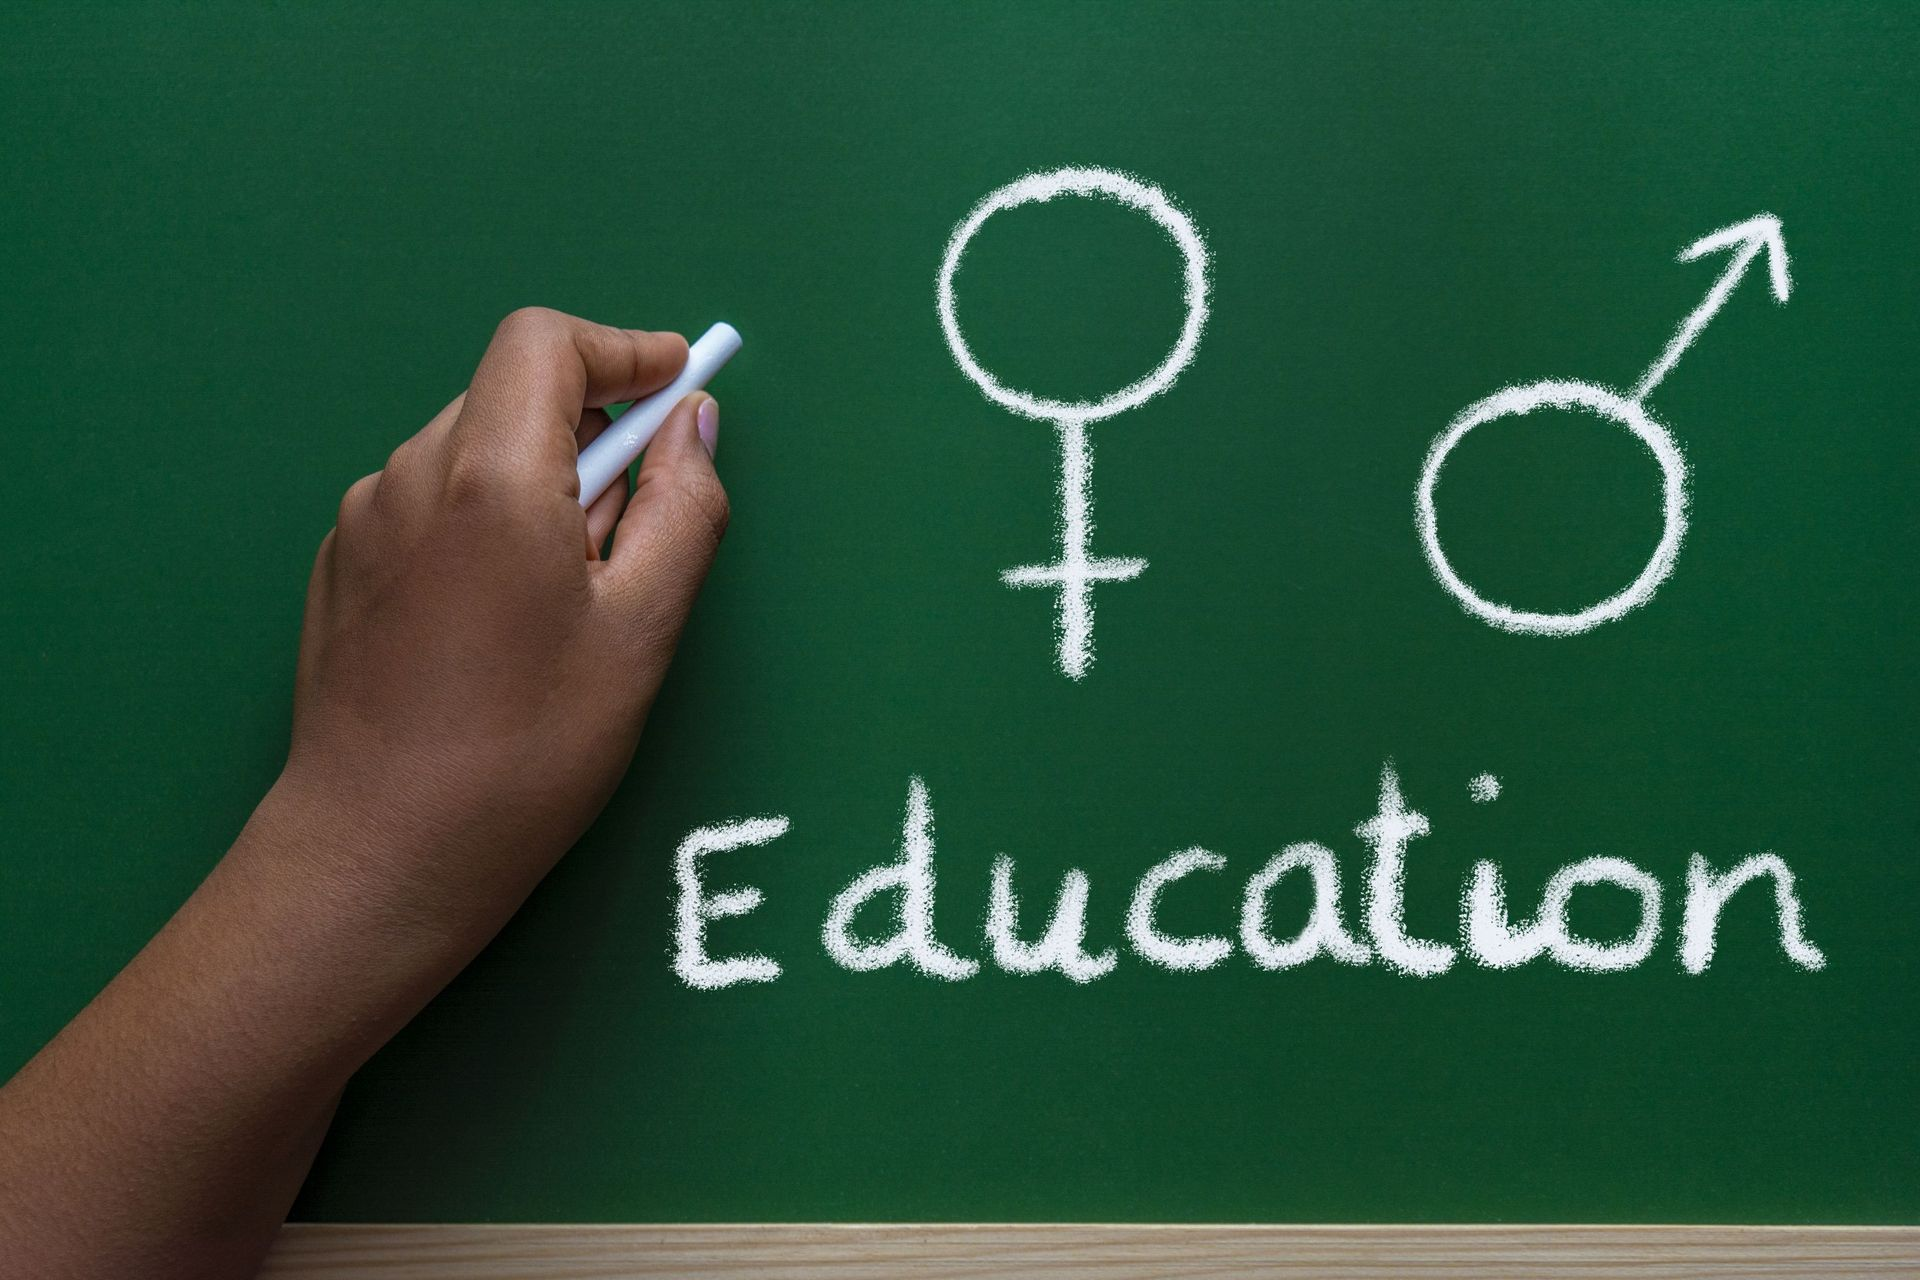
\includegraphics[scale=0.07]{education_sexe.jpg}
      \end{center}
    \column{0.6\textwidth}
      Avec un.e partenaire, lisez à tour de rôle le texte aux pages 48 et 49 dans le manuel intitulé \emph{<<Théorie du genre>> au lycée, la crainte de dérives}.
      Après chaque paragraphe, arrêtez pour en discuter.
      Qu'est-ce que vous avez compris du paragraphe?
      Quels sont vos commentaires des idées présentées dans le paragraphe?
  \end{columns}
\end{frame}